\documentclass{beamer}
%\usetheme{Goettingen}
%\usetheme{Singapore}
\usetheme{Darmstadt}
\usecolortheme{seahorse}

\AtBeginSection[]{
	\begin{frame}
		\vfill
		\centering
		\begin{beamercolorbox}[sep=8pt,center,shadow=true,rounded=true]{title}
			\usebeamerfont{title}\insertsectionhead\par%
		\end{beamercolorbox}
		\vfill
	\end{frame}
}

\usepackage[utf8]{inputenc}
\usepackage[spanish, es-tabla]{babel}


% Fracciones más grandes
\newcommand\ddfrac[2]{\frac{\displaystyle #1}{\displaystyle #2}}



%Information to be included in the title page:
\title{Determinación de Órbitas Elípticas}
\subtitle{El Método de Laplace}
\author{Simón López Vico}
\institute{Doble Grado en Matemáticas e Ingeniería Informática\\Universidad de Granada}
\date{Septiembre de 2020}


\begin{document}

\frame{\titlepage}

\begin{frame}{Índice}
\tableofcontents
\end{frame}

\section{Introducción}

\begin{frame}
\begin{figure}[H]
\centering
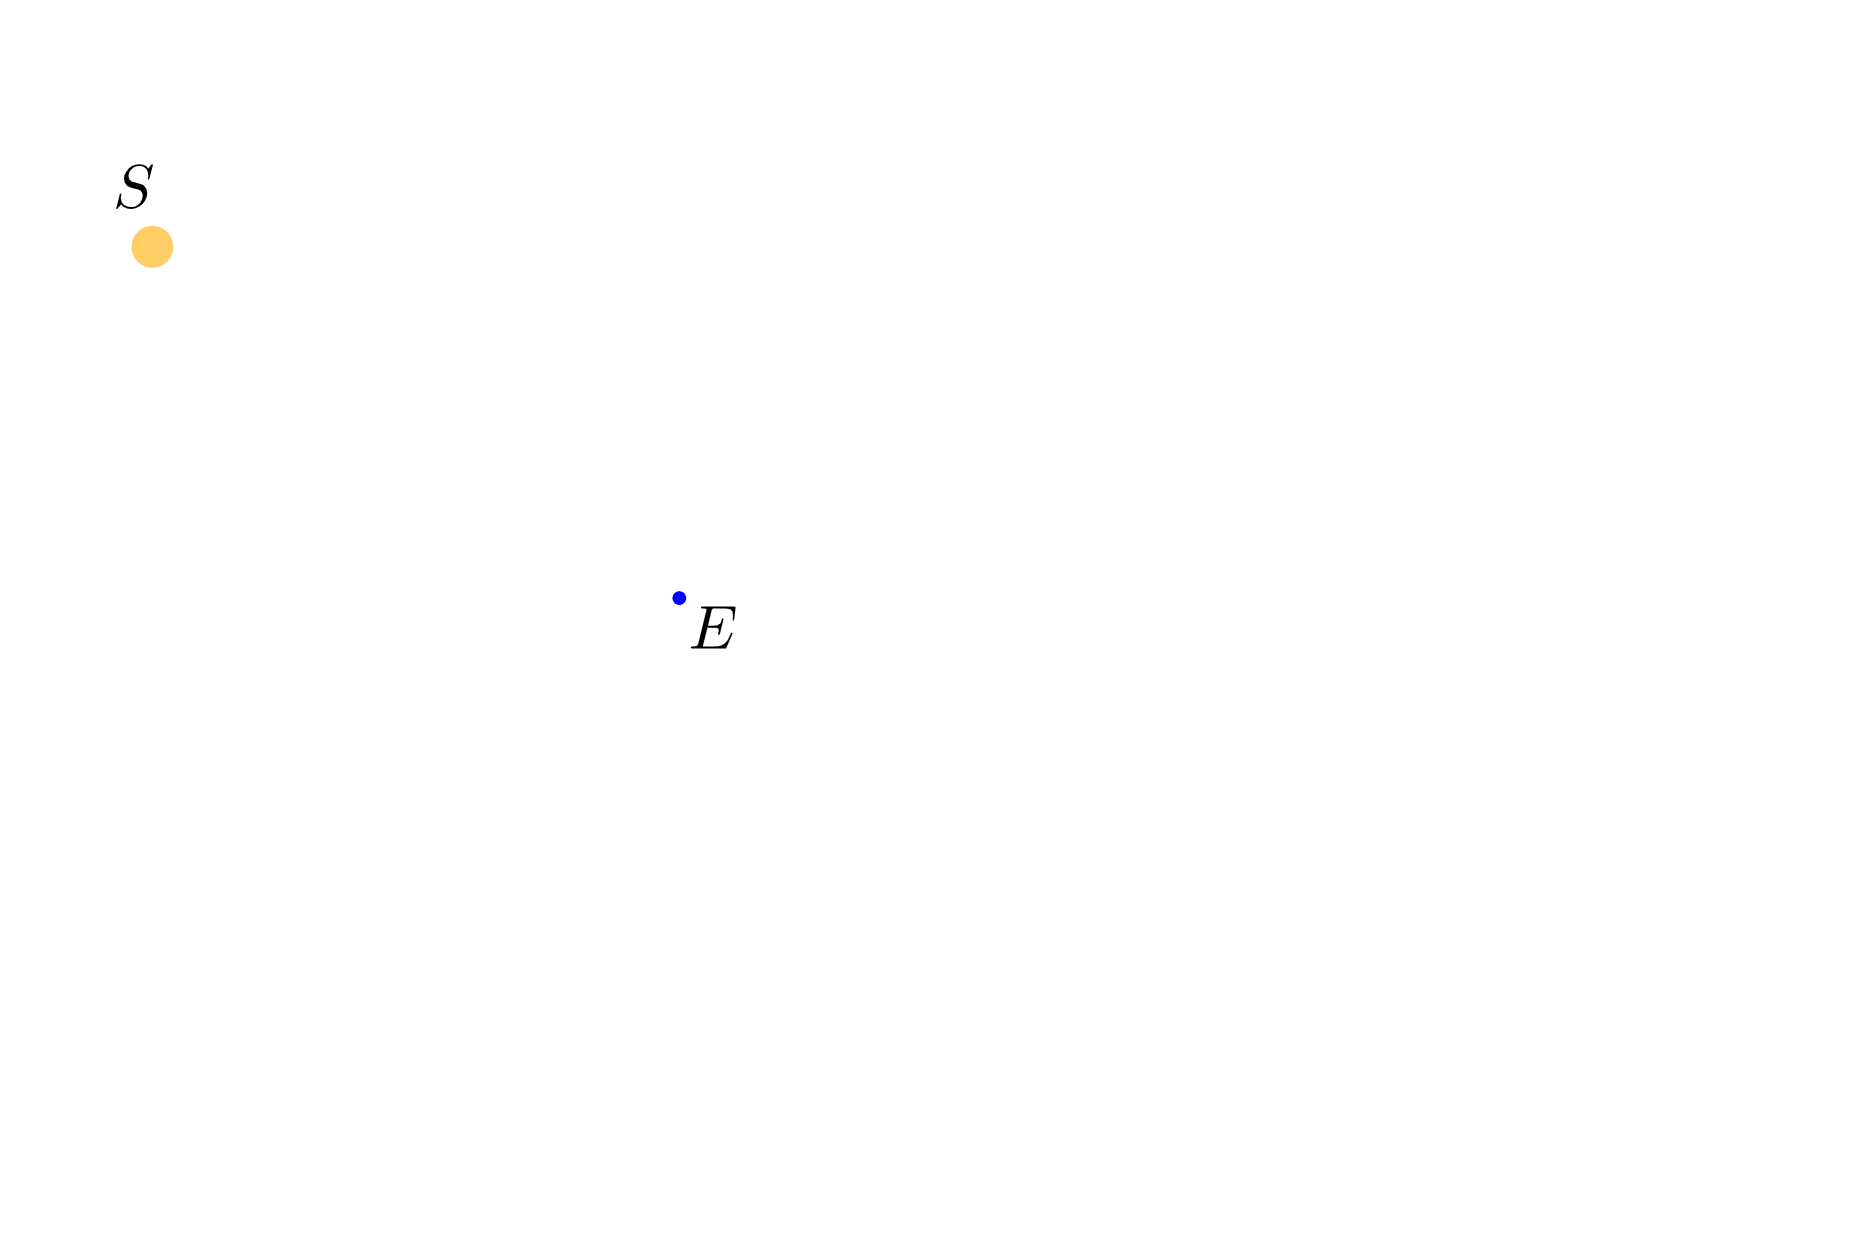
\includegraphics[scale=0.15]{images/problem_construct_1.png}
\end{figure}
\end{frame}

\begin{frame}
\begin{figure}[H]
\centering
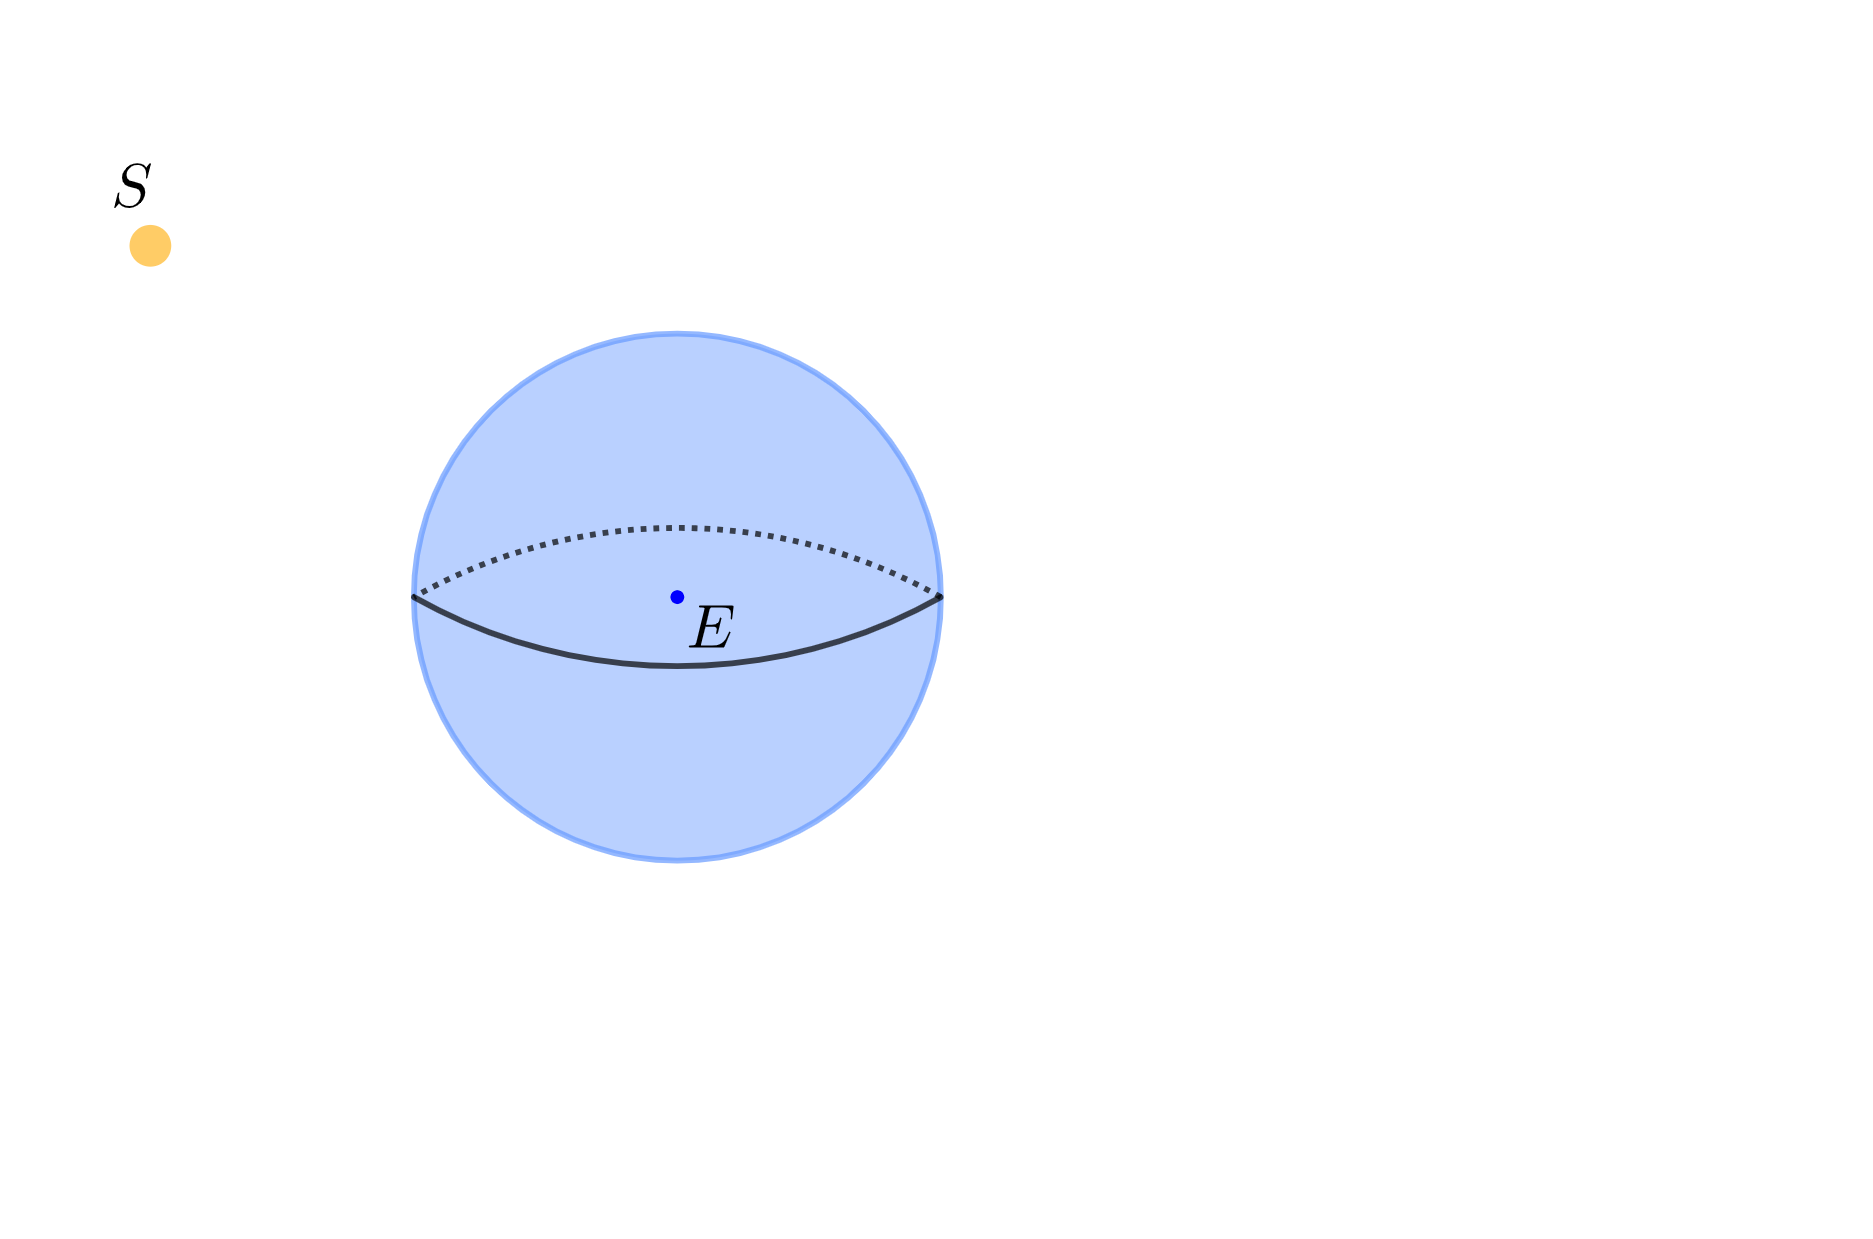
\includegraphics[scale=0.15]{images/problem_construct_2.png}
\end{figure}
\end{frame}

\begin{frame}
\begin{figure}[H]
\centering
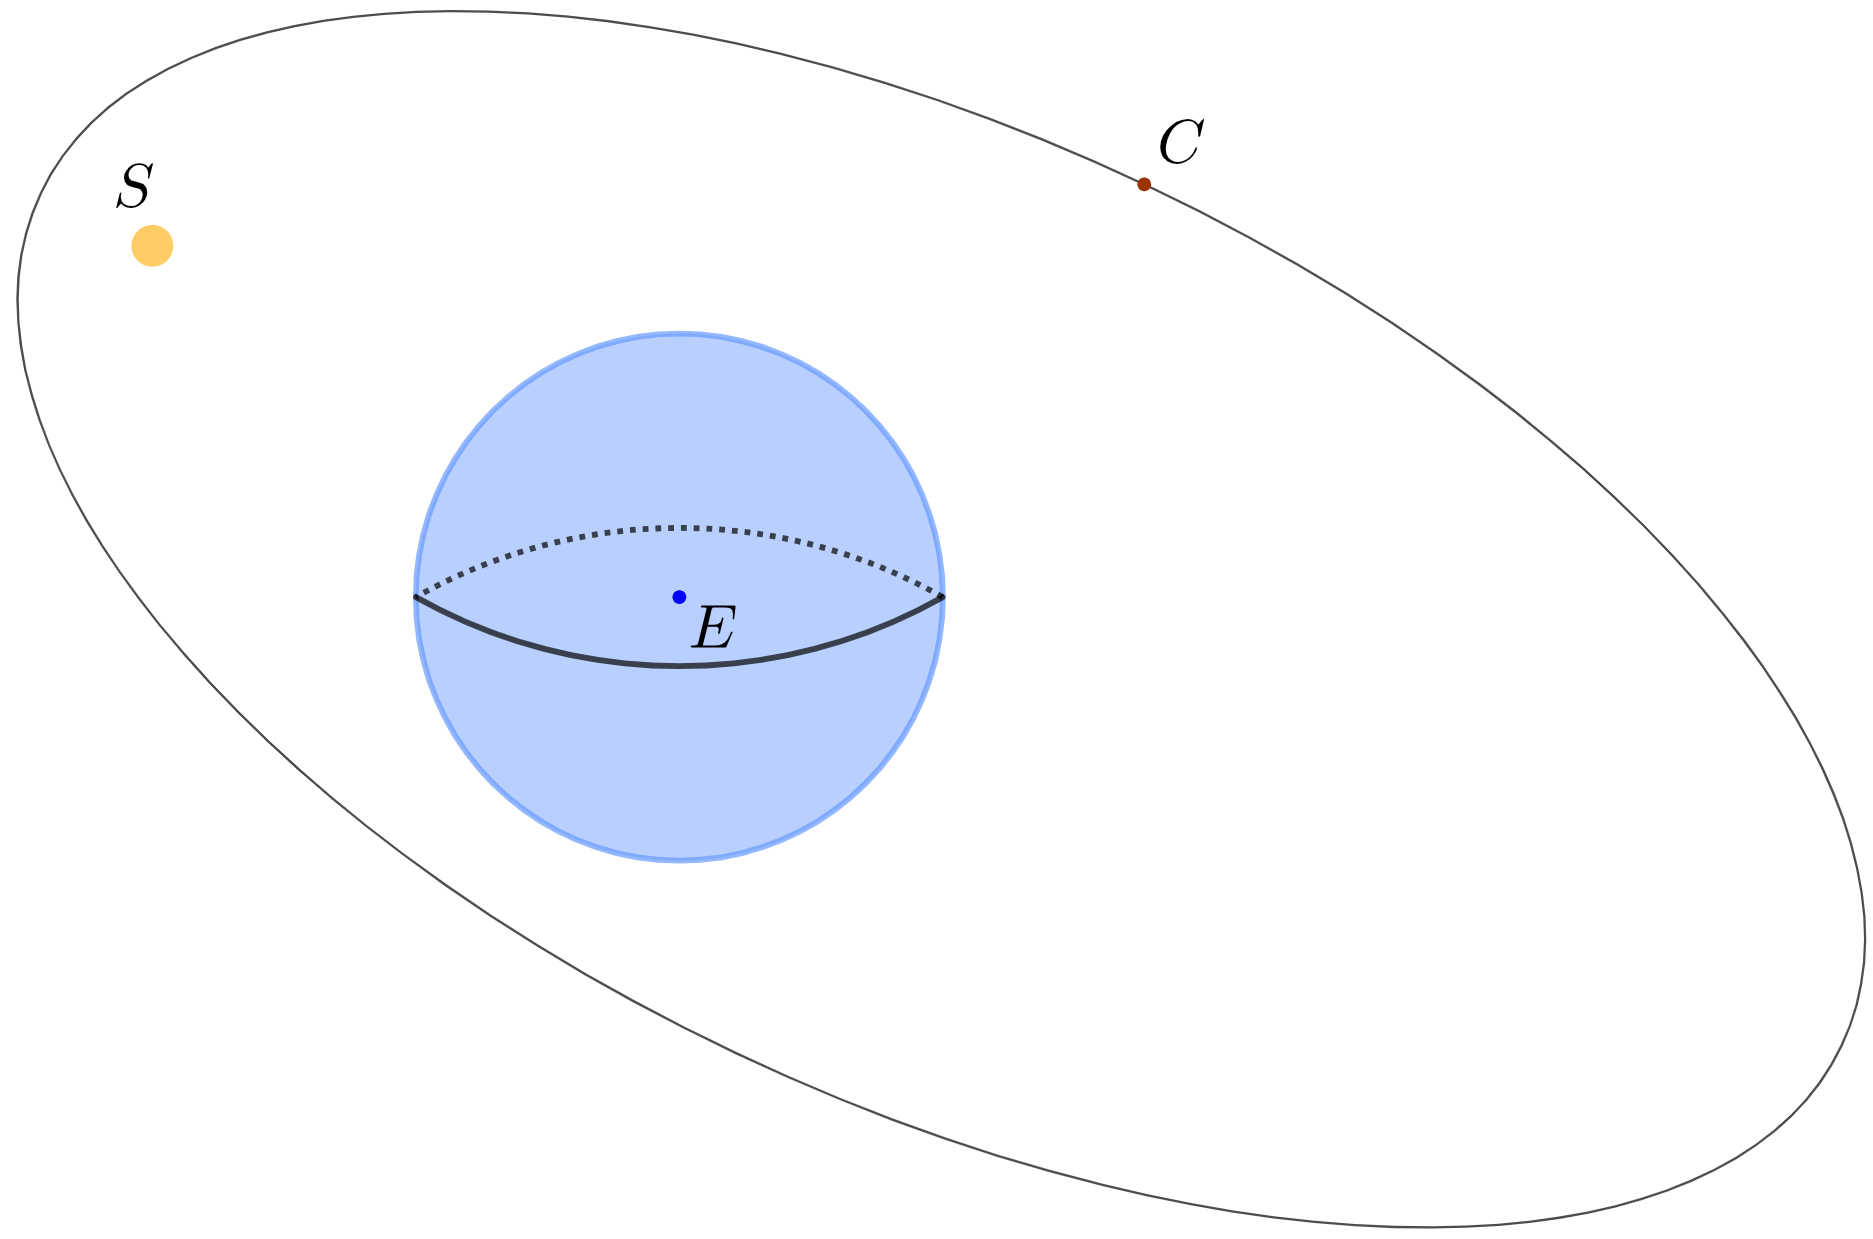
\includegraphics[scale=0.15]{images/problem_construct_3.png}
\end{figure}
\end{frame}


\section{El Método de Laplace}

\begin{frame}
\frametitle{Aproximando las derivadas}
Tres observaciones: $(\lambda_1,\mu_1,\nu_1)$, $(\lambda_2,\mu_2,\nu_2)$, $(\lambda_3,\mu_3,\nu_3)$.\pause
\vspace{0.66666cm}

\textbf{Diferencia regresiva} ($t_2>t_1$)
\[
\lambda'_{12}=\frac{\lambda_2-\lambda_1}{t_2-t_1}
\]

\textbf{Diferencia progresiva} ($t_2<t_3$)
\[
\lambda'_{23}=\frac{\lambda_3-\lambda_2}{t_3-t_2}
\]

\textbf{Diferencia centrada} ($t_2-t_1=t_3-t_2$)
\[
\lambda'_{2}=\frac{\lambda'_{12}+\lambda'_{23}}{2}
\]

\end{frame}

\begin{frame}{Cálculo de las distancias}
\begin{figure}[H]
\centering
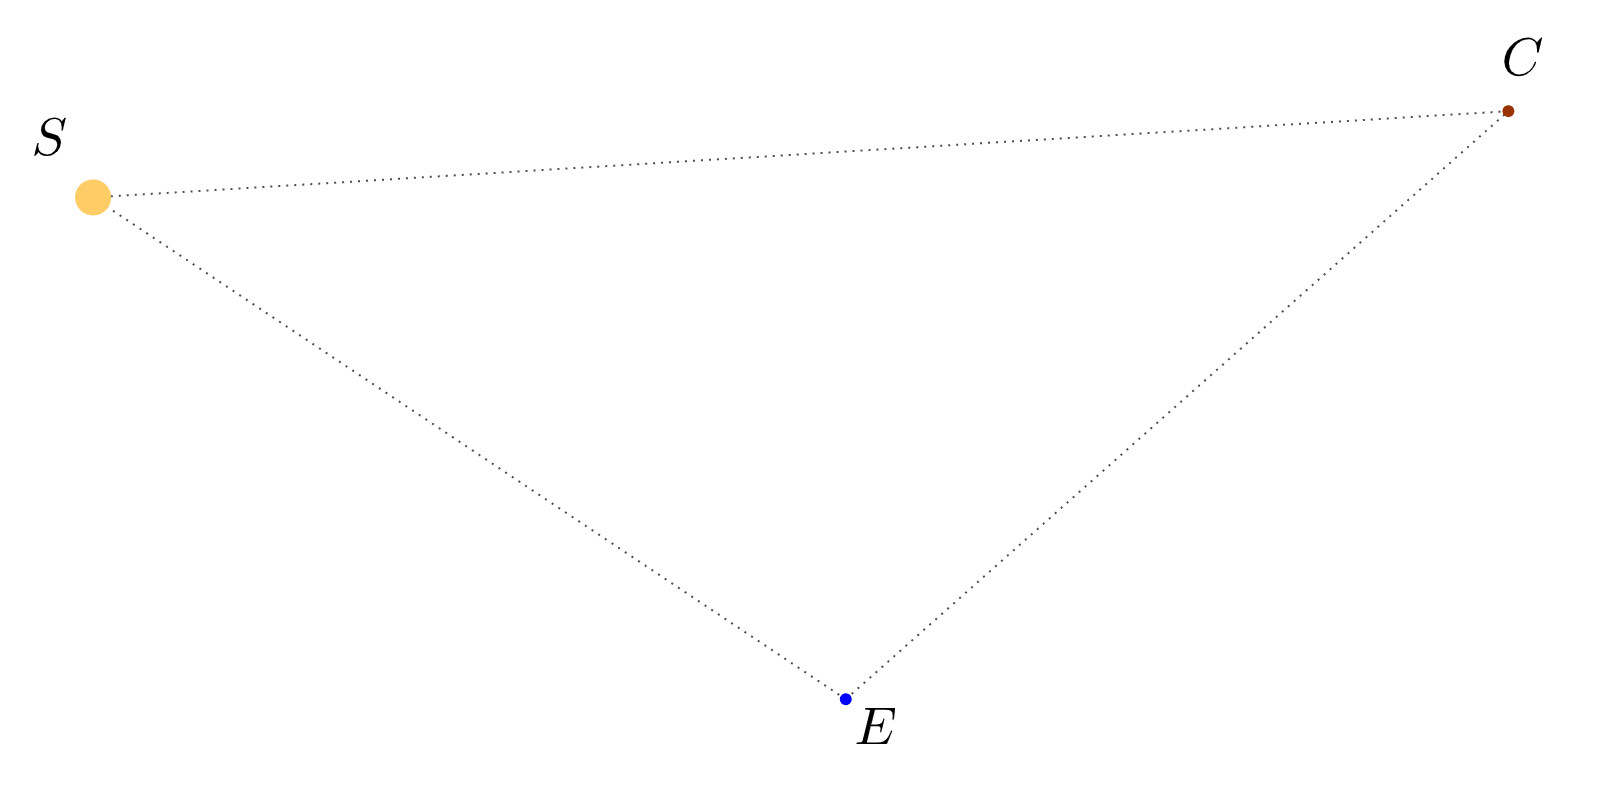
\includegraphics[scale=0.2]{images/triangle_tfg.png}
\end{figure}
\end{frame}

\begin{frame}
Soluciones para $\phi$:
\[
\sin^4{\phi}=M\sin{(\phi + m)}
\]
\vspace{0.6666cm}
\pause

Condiciones: \hspace{0.5cm}
$
\left\{
\begin{array}{l}
\phi\in(0,\pi)\\
\phi<\pi-\psi
\end{array}
\right.
$
\end{frame}

\begin{frame}{Valores para $\phi$}
\begin{figure}[H]
\centering
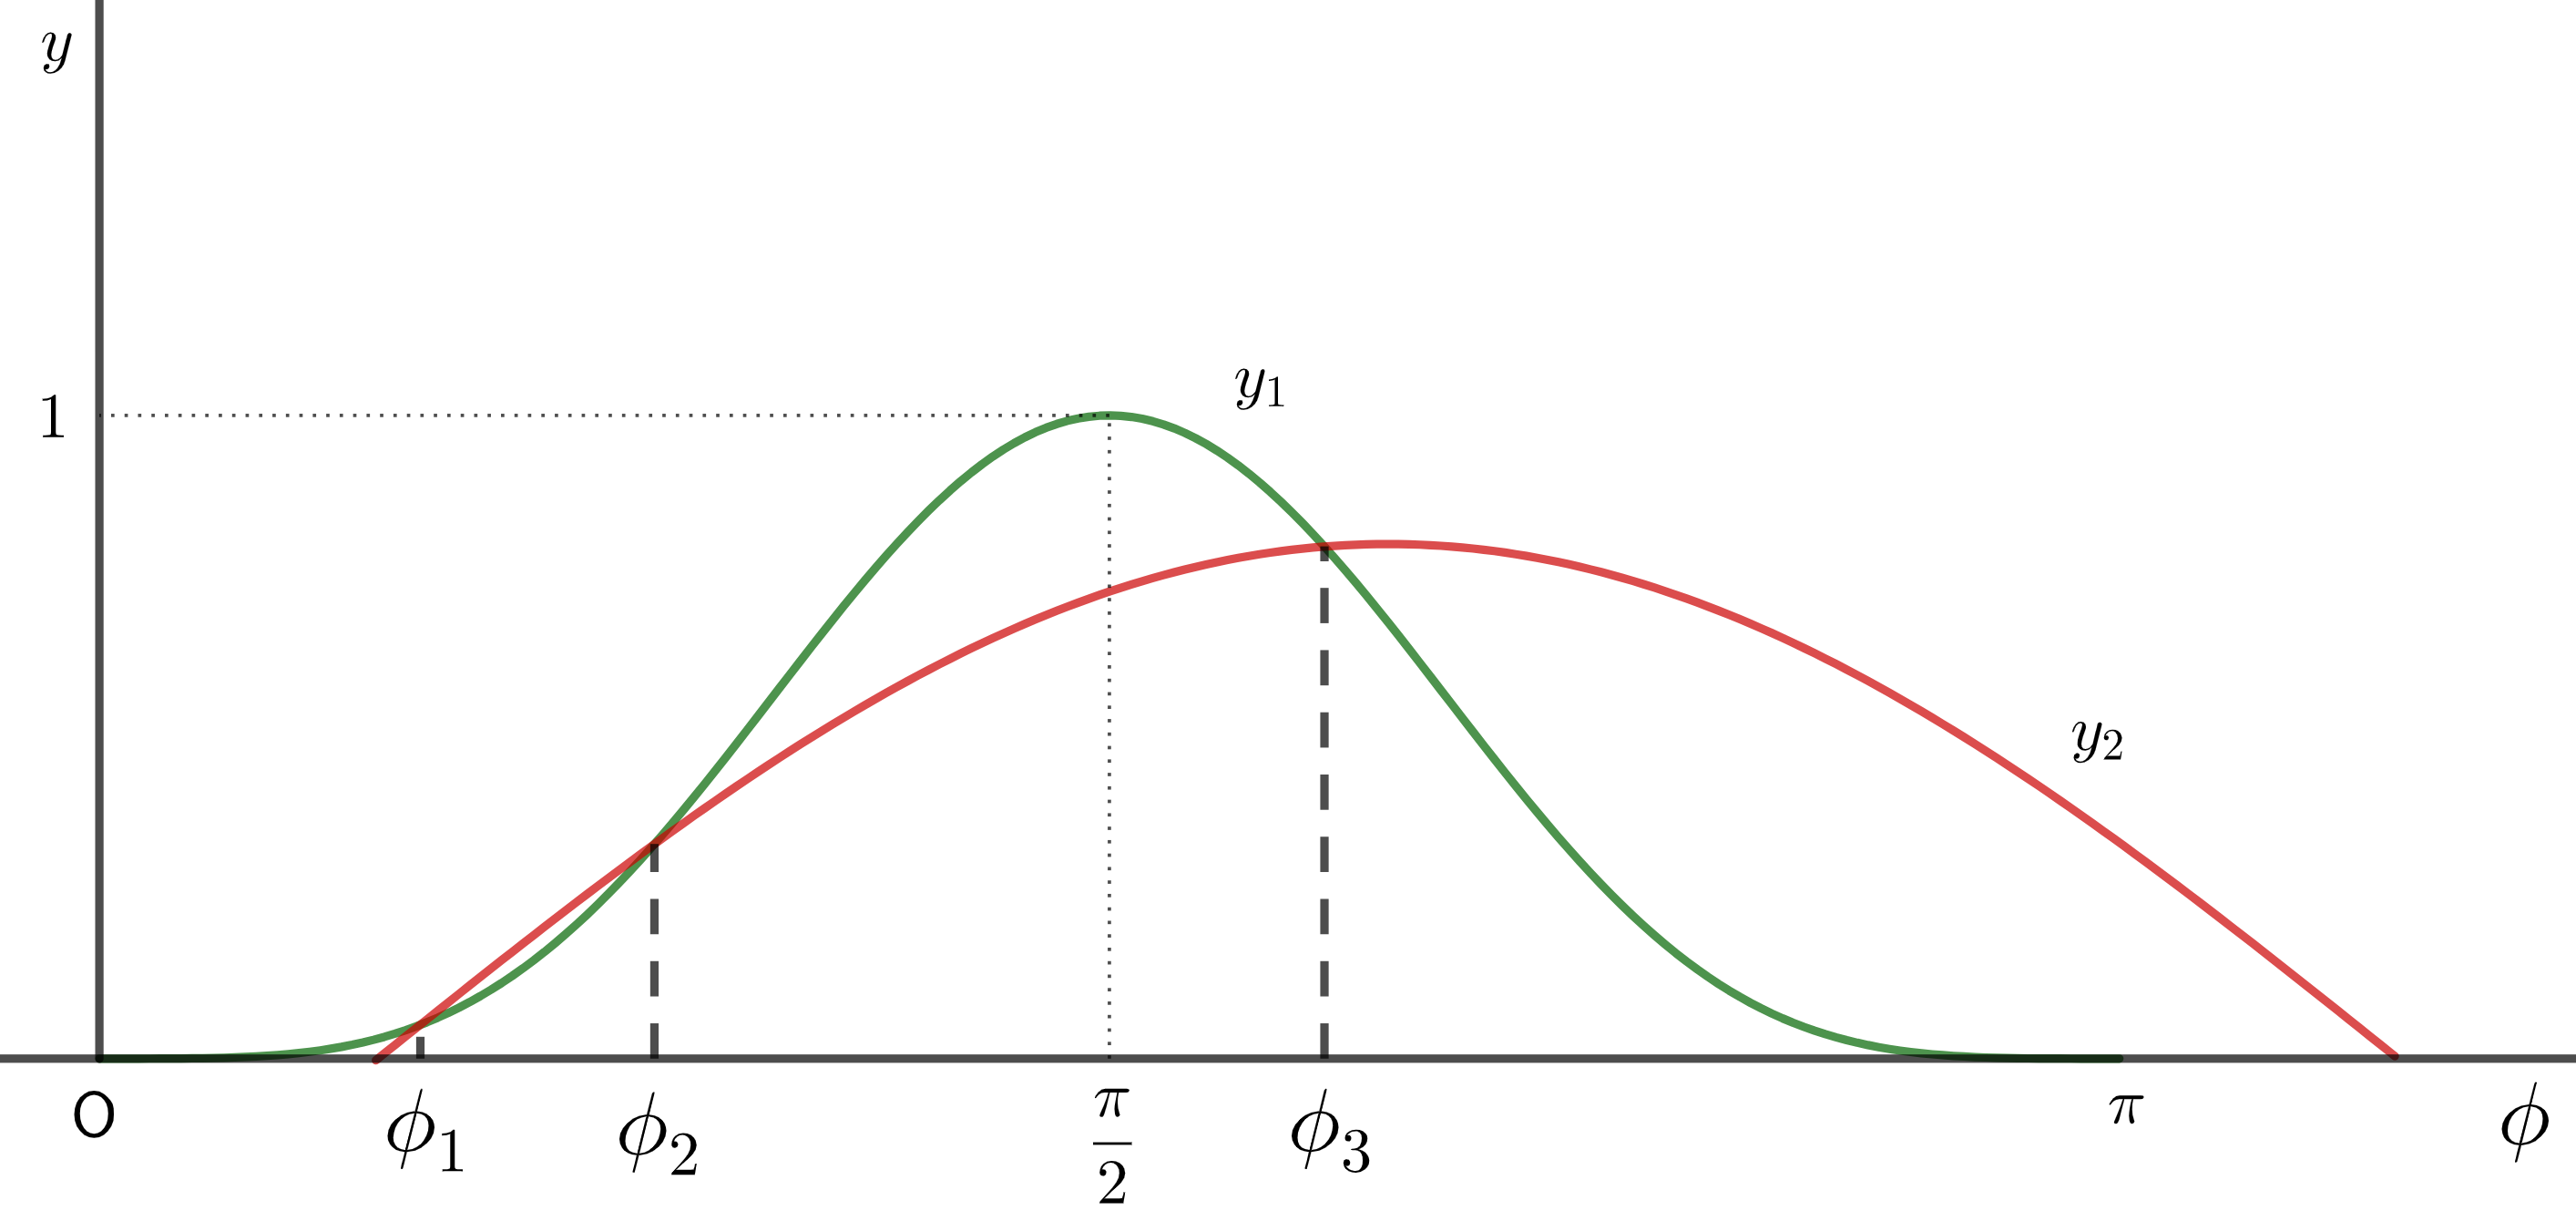
\includegraphics[scale=0.1]{images/phi_solution_m_negative_M_near_1.png}
\end{figure}

\end{frame}

\begin{frame}{Utilizamos los valores calculados}


\[\rho=R\ddfrac{\sin{(\psi+\phi)}}{\sin{\psi}}
\hspace{2cm}
\rho'=\ddfrac{D_2}{D}\left(\ddfrac{1}{R^3}-\ddfrac{1}{r^3}\right)\]\\
\vspace{1cm}

\pause
\begin{columns}
\column[]{0.35\textwidth}
\textbf{Posición:}\\
\vspace{0.4cm}
$
\left\{
\begin{array}{l}
	x=\rho\lambda-X\\
	y=\rho\mu-Y\\
	z=\rho\nu-Z
\end{array}
\right.
$
\column[]{0.35\textwidth}
\textbf{Velocidad:}\\
\vspace{0.4cm}
$
\left\{
\begin{array}{l}
	x'=\rho'\lambda+\rho\lambda'-X'\\
	y'=\rho'\mu+\rho\mu'-Y'\\
	z'=\rho'\nu+\rho\nu'-Z'
\end{array}
\right.
$
\end{columns}
\end{frame}

\section{Órbita completa del cuerpo}
\begin{frame}{Elementos orbitales}
Utilizando $r=(x,y,z)$ y $v=r'$ podemos obtener $(a,e,i,\omega,\Omega)$.\\
\pause
\vspace{1cm}
\textbf{Elipse:}
\hspace{0.75cm}
$
(a\cos{\theta}+ae, a\sqrt{1-e^2}\sin{\theta}, 0), \; \; \; \; \theta\in(0,2\pi)
$
\end{frame}


\begin{frame}{Posición de la órbita}
\begin{figure}[H]
\centering
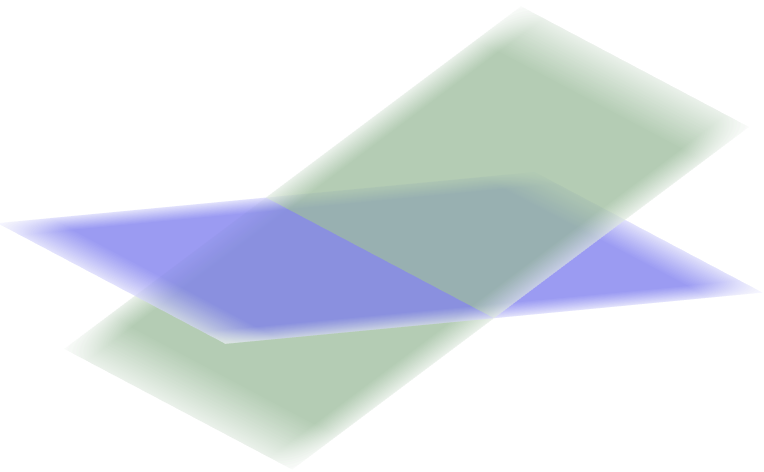
\includegraphics[scale=0.41]{images/inclinacion.png}
\end{figure}
\end{frame}

\section{Bondad del método}

\begin{frame}{Herramientas para el desarrollo}
\begin{itemize}
\item \textbf{Python:} Numpy, Matplotlib, Astropy, etc.
\item \textbf{Tkinter}
\item \textbf{Jet Propulsion Laboratory} (JPL)
\end{itemize}
\end{frame}

\begin{frame}{Cuerpos lejanos}
\textbf{Plutón} (999), observaciones 6 de marzo, 6 de abril, 6 de mayo.
\begin{columns}
\column[]{0.5\textwidth}
	\begin{table}[]
	\centering
	\resizebox{4cm}{!}{%
	\begin{tabular}{ccc}
	    & Real         & Aproximado   \\ \hline
	$x$ & 13.26236291  & 13.59730661  \\ \hline
	$y$ & -31.31779618 & -32.05011445 \\ \hline
	$z$ & -0.48455854  & -0.4966634  
	\end{tabular}%
	}
	\end{table}
	
	\begin{table}[H]
	\centering
	\resizebox{4cm}{!}{%
	\begin{tabular}{ccc}
	     & Real        & Aproximado  \\ \hline
	$x'$ & 0.0029688   & 0.00291106  \\ \hline
	$y'$ & 0.00056318  & 0.00065941  \\ \hline
	$z'$ & -0.00090387 & -0.00093223
	\end{tabular}%
	}
	\end{table}

\column[]{0.5\textwidth}
	\begin{figure}[H]
	\centering
	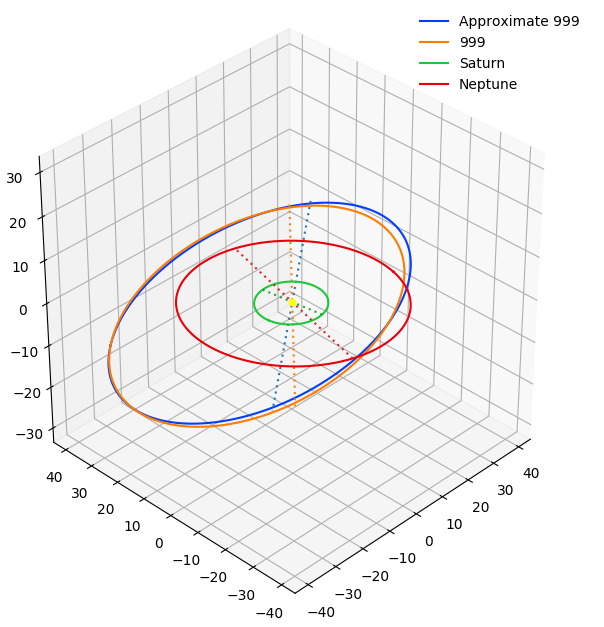
\includegraphics[scale=0.25]{images/plot_pluto_ok.png}
	\end{figure}
\end{columns}
\end{frame}

\begin{frame}{Cuerpos muy excéntricos}
\textbf{Neowise} (DES=2020 F3), observaciones con 8 horas de diferencia.
\begin{columns}
\column[]{0.5\textwidth}
	\begin{table}[]
	\centering
	\resizebox{4cm}{!}{%
	\begin{tabular}{ccc}
	    & Real         & Aproximado   \\ \hline
	$x$ & 0.16652972   & 0.16854806   \\ \hline
	$y$ & -0.24402154  & -0.25029356  \\ \hline
	$z$ & 0.32665628   & 0.32362519 
	\end{tabular}%
	}
	\end{table}
	
	\begin{table}[H]
	\centering
	\resizebox{4cm}{!}{%
	\begin{tabular}{ccc}
	     & Real        & Aproximado  \\ \hline
	$x'$ & -0.01084886 & -0.0106734  \\ \hline
	$y'$ & -0.03392851 & -0.03331783 \\ \hline
	$z'$ & 0.00860642  & 0.00864502
	\end{tabular}%
	}
	\end{table}
	
\column[]{0.5\textwidth}
	\begin{figure}[H]
	\centering
	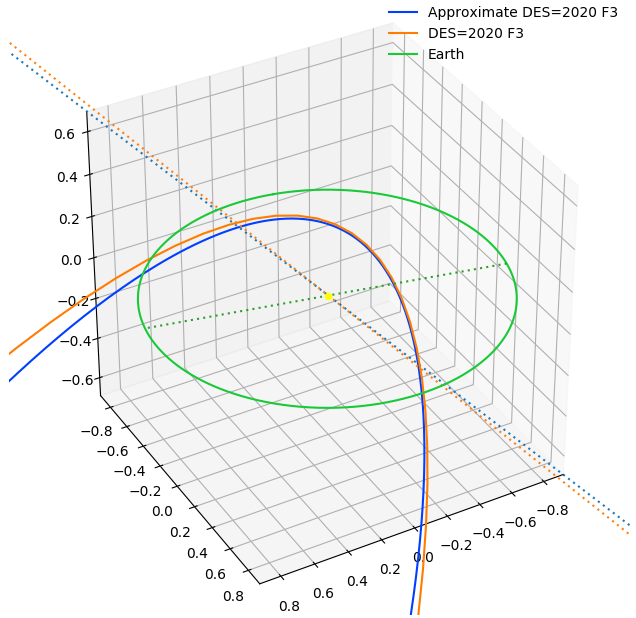
\includegraphics[scale=0.25]{images/neowise_close.png}
	\end{figure}
\end{columns}
\end{frame}

\begin{frame}
\begin{columns}
\column[]{0.5\textwidth}
	\begin{figure}[H]
	\centering
	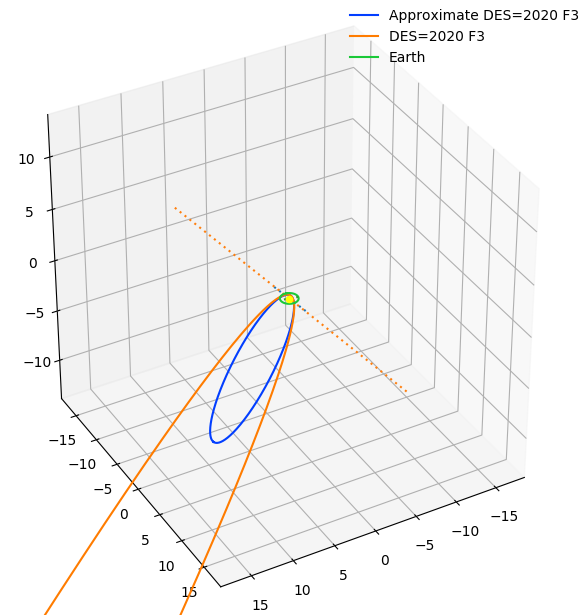
\includegraphics[scale=0.25]{images/neowise_far.png}
	\end{figure}
\column[]{0.5\textwidth}
\begin{table}[H]
\centering
\resizebox{5cm}{!}{%
\begin{tabular}{ccc}
         & Real            & Aproximado      \\ \hline
$e$      & 0.9992401080381 & 0.9623385094824 \\ \hline
$i$      & 128.9372837890  & 129.87582386324 \\ \hline
$\omega$ & 37.28105014282  & 34.302810750239 \\ \hline
$\Omega$ & 61.01063124644  & 60.32375719162
\end{tabular}%
}
\end{table}

\vspace{0.75cm}
\begin{small}
\begin{center}
	$a_{real}=387.7566248050 \text{UA}$\\
	$a_{aprox}=7.640204712942 \text{UA}$
\end{center}
\end{small}
\end{columns}
\end{frame}


\section{Conclusiones}

\begin{frame}{Conclusiones}
\begin{itemize}
\item El método de Laplace obtiene buena aproximación.
\item Cuerpos cercanos $\longrightarrow$ observaciones cercanas.\\Cuerpos lejanos $\longrightarrow$ observaciones lejanas.
\item Implementación software funciona al completo.
\end{itemize}
\end{frame}

\begin{frame}

\vspace{1cm}

\begin{center}
\Large Muchas gracias por su atención\\
\vspace{0.7cm}
\footnotesize Correo de contacto: \textit{simondelosbros@correo.ugr.es}
\end{center}

\end{frame}


\end{document}